
%% bare_conf.tex
%% V1.3
%% 2007/01/11
%% by Michael Shell
%% See:
%% http://www.michaelshell.org/
%% for current contact information.
%%
%% This is a skeleton file demonstrating the use of IEEEtran.cls
%% (requires IEEEtran.cls version 1.7 or later) with an IEEE conference paper.
%%
%% Support sites:
%% http://www.michaelshell.org/tex/ieeetran/
%% http://www.ctan.org/tex-archive/macros/latex/contrib/IEEEtran/
%% and
%% http://www.ieee.org/

%%*************************************************************************
%% Legal Notice:
%% This code is offered as-is without any warranty either expressed or
%% implied; without even the implied warranty of MERCHANTABILITY or
%% FITNESS FOR A PARTICULAR PURPOSE! 
%% User assumes all risk.
%% In no event shall IEEE or any contributor to this code be liable for
%% any damages or losses, including, but not limited to, incidental,
%% consequential, or any other damages, resulting from the use or misuse
%% of any information contained here.
%%
%% All comments are the opinions of their respective authors and are not
%% necessarily endorsed by the IEEE.
%%
%% This work is distributed under the LaTeX Project Public License (LPPL)
%% ( http://www.latex-project.org/ ) version 1.3, and may be freely used,
%% distributed and modified. A copy of the LPPL, version 1.3, is included
%% in the base LaTeX documentation of all distributions of LaTeX released
%% 2003/12/01 or later.
%% Retain all contribution notices and credits.
%% ** Modified files should be clearly indicated as such, including  **
%% ** renaming them and changing author support contact information. **
%%
%% File list of work: IEEEtran.cls, IEEEtran_HOWTO.pdf, bare_adv.tex,
%%                    bare_conf.tex, bare_jrnl.tex, bare_jrnl_compsoc.tex
%%*************************************************************************

% *** Authors should verify (and, if needed, correct) their LaTeX system  ***
% *** with the testflow diagnostic prior to trusting their LaTeX platform ***
% *** with production work. IEEE's font choices can trigger bugs that do  ***
% *** not appear when using other class files.                            ***
% The testflow support page is at:
% http://www.michaelshell.org/tex/testflow/



% Note that the a4paper option is mainly intended so that authors in
% countries using A4 can easily print to A4 and see how their papers will
% look in print - the typesetting of the document will not typically be
% affected with changes in paper size (but the bottom and side margins will).
% Use the testflow package mentioned above to verify correct handling of
% both paper sizes by the user's LaTeX system.
%
% Also note that the "draftcls" or "draftclsnofoot", not "draft", option
% should be used if it is desired that the figures are to be displayed in
% draft mode.
%
\documentclass[conference]{IEEEtran}
% Add the compsoc option for Computer Society conferences.
%
% If IEEEtran.cls has not been installed into the LaTeX system files,
% manually specify the path to it like:
% \documentclass[conference]{../sty/IEEEtran}





% Some very useful LaTeX packages include:
% (uncomment the ones you want to load)


% *** MISC UTILITY PACKAGES ***
%
%\usepackage{ifpdf}
% Heiko Oberdiek's ifpdf.sty is very useful if you need conditional
% compilation based on whether the output is pdf or dvi.
% usage:
% \ifpdf
%   % pdf code
% \else
%   % dvi code
% \fi
% The latest version of ifpdf.sty can be obtained from:
% http://www.ctan.org/tex-archive/macros/latex/contrib/oberdiek/
% Also, note that IEEEtran.cls V1.7 and later provides a builtin
% \ifCLASSINFOpdf conditional that works the same way.
% When switching from latex to pdflatex and vice-versa, the compiler may
% have to be run twice to clear warning/error messages.






% *** CITATION PACKAGES ***
%
%\usepackage{cite}
% cite.sty was written by Donald Arseneau
% V1.6 and later of IEEEtran pre-defines the format of the cite.sty package
% \cite{} output to follow that of IEEE. Loading the cite package will
% result in citation numbers being automatically sorted and properly
% "compressed/ranged". e.g., [1], [9], [2], [7], [5], [6] without using
% cite.sty will become [1], [2], [5]--[7], [9] using cite.sty. cite.sty's
% \cite will automatically add leading space, if needed. Use cite.sty's
% noadjust option (cite.sty V3.8 and later) if you want to turn this off.
% cite.sty is already installed on most LaTeX systems. Be sure and use
% version 4.0 (2003-05-27) and later if using hyperref.sty. cite.sty does
% not currently provide for hyperlinked citations.
% The latest version can be obtained at:
% http://www.ctan.org/tex-archive/macros/latex/contrib/cite/
% The documentation is contained in the cite.sty file itself.






% *** GRAPHICS RELATED PACKAGES ***
%
\ifCLASSINFOpdf
  \usepackage[pdftex]{graphicx}
  % declare the path(s) where your graphic files are
  % \graphicspath{{../pdf/}{../jpeg/}}
  % and their extensions so you won't have to specify these with
  % every instance of \includegraphics
  % \DeclareGraphicsExtensions{.pdf,.jpeg,.png}
\else
  % or other class option (dvipsone, dvipdf, if not using dvips). graphicx
  % will default to the driver specified in the system graphics.cfg if no
  % driver is specified.
  \usepackage[dvips]{graphicx}
  % declare the path(s) where your graphic files are
  % \graphicspath{{../eps/}}
  % and their extensions so you won't have to specify these with
  % every instance of \includegraphics
  % \DeclareGraphicsExtensions{.eps}
\fi
% graphicx was written by David Carlisle and Sebastian Rahtz. It is
% required if you want graphics, photos, etc. graphicx.sty is already
% installed on most LaTeX systems. The latest version and documentation can
% be obtained at: 
% http://www.ctan.org/tex-archive/macros/latex/required/graphics/
% Another good source of documentation is "Using Imported Graphics in
% LaTeX2e" by Keith Reckdahl which can be found as epslatex.ps or
% epslatex.pdf at: http://www.ctan.org/tex-archive/info/
%
% latex, and pdflatex in dvi mode, support graphics in encapsulated
% postscript (.eps) format. pdflatex in pdf mode supports graphics
% in .pdf, .jpeg, .png and .mps (metapost) formats. Users should ensure
% that all non-photo figures use a vector format (.eps, .pdf, .mps) and
% not a bitmapped formats (.jpeg, .png). IEEE frowns on bitmapped formats
% which can result in "jaggedy"/blurry rendering of lines and letters as
% well as large increases in file sizes.
%
% You can find documentation about the pdfTeX application at:
% http://www.tug.org/applications/pdftex





% *** MATH PACKAGES ***
%
\usepackage[cmex10]{amsmath}
% A popular package from the American Mathematical Society that provides
% many useful and powerful commands for dealing with mathematics. If using
% it, be sure to load this package with the cmex10 option to ensure that
% only type 1 fonts will utilized at all point sizes. Without this option,
% it is possible that some math symbols, particularly those within
% footnotes, will be rendered in bitmap form which will result in a
% document that can not be IEEE Xplore compliant!
%
% Also, note that the amsmath package sets \interdisplaylinepenalty to 10000
% thus preventing page breaks from occurring within multiline equations. Use:
%\interdisplaylinepenalty=2500
% after loading amsmath to restore such page breaks as IEEEtran.cls normally
% does. amsmath.sty is already installed on most LaTeX systems. The latest
% version and documentation can be obtained at:
% http://www.ctan.org/tex-archive/macros/latex/required/amslatex/math/





% *** SPECIALIZED LIST PACKAGES ***
%
\usepackage{algorithm}
\usepackage{algpseudocode}
% algorithmic.sty was written by Peter Williams and Rogerio Brito.
% This package provides an algorithmic environment fo describing algorithms.
% You can use the algorithmic environment in-text or within a figure
% environment to provide for a floating algorithm. Do NOT use the algorithm
% floating environment provided by algorithm.sty (by the same authors) or
% algorithm2e.sty (by Christophe Fiorio) as IEEE does not use dedicated
% algorithm float types and packages that provide these will not provide
% correct IEEE style captions. The latest version and documentation of
% algorithmic.sty can be obtained at:
% http://www.ctan.org/tex-archive/macros/latex/contrib/algorithms/
% There is also a support site at:
% http://algorithms.berlios.de/index.html
% Also of interest may be the (relatively newer and more customizable)
% algorithmicx.sty package by Szasz Janos:
% http://www.ctan.org/tex-archive/macros/latex/contrib/algorithmicx/




% *** ALIGNMENT PACKAGES ***
%
%\usepackage{array}
% Frank Mittelbach's and David Carlisle's array.sty patches and improves
% the standard LaTeX2e array and tabular environments to provide better
% appearance and additional user controls. As the default LaTeX2e table
% generation code is lacking to the point of almost being broken with
% respect to the quality of the end results, all users are strongly
% advised to use an enhanced (at the very least that provided by array.sty)
% set of table tools. array.sty is already installed on most systems. The
% latest version and documentation can be obtained at:
% http://www.ctan.org/tex-archive/macros/latex/required/tools/


%\usepackage{mdwmath}
%\usepackage{mdwtab}
% Also highly recommended is Mark Wooding's extremely powerful MDW tools,
% especially mdwmath.sty and mdwtab.sty which are used to format equations
% and tables, respectively. The MDWtools set is already installed on most
% LaTeX systems. The lastest version and documentation is available at:
% http://www.ctan.org/tex-archive/macros/latex/contrib/mdwtools/


% IEEEtran contains the IEEEeqnarray family of commands that can be used to
% generate multiline equations as well as matrices, tables, etc., of high
% quality.


%\usepackage{eqparbox}
% Also of notable interest is Scott Pakin's eqparbox package for creating
% (automatically sized) equal width boxes - aka "natural width parboxes".
% Available at:
% http://www.ctan.org/tex-archive/macros/latex/contrib/eqparbox/





% *** SUBFIGURE PACKAGES ***
%\usepackage[tight,footnotesize]{subfigure}
% subfigure.sty was written by Steven Douglas Cochran. This package makes it
% easy to put subfigures in your figures. e.g., "Figure 1a and 1b". For IEEE
% work, it is a good idea to load it with the tight package option to reduce
% the amount of white space around the subfigures. subfigure.sty is already
% installed on most LaTeX systems. The latest version and documentation can
% be obtained at:
% http://www.ctan.org/tex-archive/obsolete/macros/latex/contrib/subfigure/
% subfigure.sty has been superceeded by subfig.sty.



%\usepackage[caption=false]{caption}
%\usepackage[font=footnotesize]{subfig}
% subfig.sty, also written by Steven Douglas Cochran, is the modern
% replacement for subfigure.sty. However, subfig.sty requires and
% automatically loads Axel Sommerfeldt's caption.sty which will override
% IEEEtran.cls handling of captions and this will result in nonIEEE style
% figure/table captions. To prevent this problem, be sure and preload
% caption.sty with its "caption=false" package option. This is will preserve
% IEEEtran.cls handing of captions. Version 1.3 (2005/06/28) and later 
% (recommended due to many improvements over 1.2) of subfig.sty supports
% the caption=false option directly:
%\usepackage[caption=false,font=footnotesize]{subfig}
%
% The latest version and documentation can be obtained at:
% http://www.ctan.org/tex-archive/macros/latex/contrib/subfig/
% The latest version and documentation of caption.sty can be obtained at:
% http://www.ctan.org/tex-archive/macros/latex/contrib/caption/




% *** FLOAT PACKAGES ***
%
%\usepackage{fixltx2e}
% fixltx2e, the successor to the earlier fix2col.sty, was written by
% Frank Mittelbach and David Carlisle. This package corrects a few problems
% in the LaTeX2e kernel, the most notable of which is that in current
% LaTeX2e releases, the ordering of single and double column floats is not
% guaranteed to be preserved. Thus, an unpatched LaTeX2e can allow a
% single column figure to be placed prior to an earlier double column
% figure. The latest version and documentation can be found at:
% http://www.ctan.org/tex-archive/macros/latex/base/



%\usepackage{stfloats}
% stfloats.sty was written by Sigitas Tolusis. This package gives LaTeX2e
% the ability to do double column floats at the bottom of the page as well
% as the top. (e.g., "\begin{figure*}[!b]" is not normally possible in
% LaTeX2e). It also provides a command:
%\fnbelowfloat
% to enable the placement of footnotes below bottom floats (the standard
% LaTeX2e kernel puts them above bottom floats). This is an invasive package
% which rewrites many portions of the LaTeX2e float routines. It may not work
% with other packages that modify the LaTeX2e float routines. The latest
% version and documentation can be obtained at:
% http://www.ctan.org/tex-archive/macros/latex/contrib/sttools/
% Documentation is contained in the stfloats.sty comments as well as in the
% presfull.pdf file. Do not use the stfloats baselinefloat ability as IEEE
% does not allow \baselineskip to stretch. Authors submitting work to the
% IEEE should note that IEEE rarely uses double column equations and
% that authors should try to avoid such use. Do not be tempted to use the
% cuted.sty or midfloat.sty packages (also by Sigitas Tolusis) as IEEE does
% not format its papers in such ways.





% *** PDF, URL AND HYPERLINK PACKAGES ***
%
%\usepackage{url}
% url.sty was written by Donald Arseneau. It provides better support for
% handling and breaking URLs. url.sty is already installed on most LaTeX
% systems. The latest version can be obtained at:
% http://www.ctan.org/tex-archive/macros/latex/contrib/misc/
% Read the url.sty source comments for usage information. Basically,
% \url{my_url_here}.





% *** Do not adjust lengths that control margins, column widths, etc. ***
% *** Do not use packages that alter fonts (such as pslatex).         ***
% There should be no need to do such things with IEEEtran.cls V1.6 and later.
% (Unless specifically asked to do so by the journal or conference you plan
% to submit to, of course. )


% correct bad hyphenation here
\hyphenation{op-tical net-works semi-conduc-tor}

\usepackage{listings}
\usepackage{comment}
\usepackage{paralist}
\usepackage{multirow}
\usepackage{multicol}
\usepackage{soul}
\usepackage{verbatim}
\usepackage{url}
\usepackage{color}
\usepackage{paralist}
%\usepackage[bookmarks=false]{hyperref}

\newcommand{\figref}[1]{Figure~\ref{#1}}
\newcommand{\algoref}[1]{Algorithm~\ref{#1}}
\newcommand{\tableref}[1]{Table~\ref{#1}}
\newcommand{\secref}[1]{Section~\ref{#1}}
\newcommand{\lineref}[1]{Line~\ref{#1}}

\definecolor{dkgreen}{rgb}{0,0.6,0}
\definecolor{gray}{rgb}{0.5,0.5,0.5}
\definecolor{mauve}{rgb}{0.58,0,0.82}

\lstset{frame=tb,
  language=Java,
  aboveskip=3mm,
  belowskip=3mm,
  showstringspaces=false,
  columns=flexible,
  basicstyle={\small\ttfamily},
  numbers=none,
  numberstyle=\tiny\color{gray},
  keywordstyle=\color{blue},
  commentstyle=\color{dkgreen},
  stringstyle=\color{mauve},
  breaklines=true,
  breakatwhitespace=true
  tabsize=2
}

% custom macros
\newcommand{\hjKwd}[1]{\texttt{#1}}
\newcommand{\hjCode}[1]{\texttt{#1}}
\newcommand{\newTerm}[1]{\textit{#1}}
\newcommand{\hjv}{HJ-V}
\newcommand{\hj}{HJ}
\newcommand{\jpf}{JPF}
\newcommand{\jpfhj}{JPF-HJ}

\newcommand{\todo}[1]{\textcolor{red}{#1}}

%theorem environments
\usepackage{mathtools}
\usepackage{amsthm}
\newtheorem{theorem}{Theorem}
\newtheorem{lemma}[theorem]{Lemma}
\newtheorem{proposition}[theorem]{Proposition}
\newtheorem{corollary}[theorem]{Corollary}
\newtheorem{definition}{Definition}

\begin{document}
%
% paper title
% can use linebreaks \\ within to get better formatting as desired
\title{Model Checking Task Parallel Programs using Gradual Permissions}

% author names and affiliations
% use a multiple column layout for up to three different
% affiliations
\author{\IEEEauthorblockN{Eric G Mercer and Peter Anderson}
\IEEEauthorblockA{Brigham Young University\\
Provo, Utah, USA\\
Email: eric.mercer,anderson.peter@byu.edu}
\and
\IEEEauthorblockN{Nick Vrvilo and Vivek Sarkar}
\IEEEauthorblockA{Rice University\\
Houston, TX, USA\\
Email: nick.vrvilo,vsarkar@rice.edu}
\thanks{This work is funded by NSF Award CCF-1302524}}

% conference papers do not typically use \thanks and this command
% is locked out in conference mode. If really needed, such as for
% the acknowledgment of grants, issue a \IEEEoverridecommandlockouts
% after \documentclass

% for over three affiliations, or if they all won't fit within the width
% of the page, use this alternative format:
% 
%\author{\IEEEauthorblockN{Michael Shell\IEEEauthorrefmark{1},
%Homer Simpson\IEEEauthorrefmark{2},
%James Kirk\IEEEauthorrefmark{3}, 
%Montgomery Scott\IEEEauthorrefmark{3} and
%Eldon Tyrell\IEEEauthorrefmark{4}}
%\IEEEauthorblockA{\IEEEauthorrefmark{1}School of Electrical and Computer Engineering\\
%Georgia Institute of Technology,
%Atlanta, Georgia 30332--0250\\ Email: see http://www.michaelshell.org/contact.html}
%\IEEEauthorblockA{\IEEEauthorrefmark{2}Twentieth Century Fox, Springfield, USA\\
%Email: homer@thesimpsons.com}
%\IEEEauthorblockA{\IEEEauthorrefmark{3}Starfleet Academy, San Francisco, California 96678-2391\\
%Telephone: (800) 555--1212, Fax: (888) 555--1212}
%\IEEEauthorblockA{\IEEEauthorrefmark{4}Tyrell Inc., 123 Replicant Street, Los Angeles, California 90210--4321}}




% use for special paper notices
%\IEEEspecialpapernotice{(Invited Paper)}




% make the title area
\maketitle


\begin{abstract}
Task parallel programming languages provide a way for creating asynchronous tasks that can run concurrently. The advantage of using task parallelism is that the programmer can write code that is independent of the underlying hardware. The runtime determines the number of processor cores that are available and the most efficient way to execute the tasks. When two or more concurrently executing tasks access a shared memory location and if at least one of the accesses is for writing, data race is observed in the program. Data races can introduce non-determinism in the program output making it important to have data race detection tools. To detect data races in task parallel programs, a new sound and complete technique based on computation graphs is presented in this work. The data race detection algorithm runs in $\mathcal{O}$(N$^2$) time where N is number of nodes in the graph. A computation graph is a directed acyclic graph that represents the execution of the program. For detecting data races, the computation graph stores shared heap locations accessed by the tasks. An algorithm for creating computation graphs augmented with memory locations accessed by the tasks is also described here. This algorithm runs in $\mathcal{O}$(N) time where N is the number of operations performed in the tasks. A scheduling algorithm that creates all possible computation graph structures for programs containing critical sections is also presented here. This work also presents an implementation of this technique for the Java implementation of the Habanero programming model. The results of this data race detector are compared to Java Pathfinder's precise race detector extension and permission regions based race detector extension. The results show a significant reduction in the time required for data race detection using this technique.
\end{abstract}
% IEEEtran.cls defaults to using nonbold math in the Abstract.
% This preserves the distinction between vectors and scalars. However,
% if the conference you are submitting to favors bold math in the abstract,
% then you can use LaTeX's standard command \boldmath at the very start
% of the abstract to achieve this. Many IEEE journals/conferences frown on
% math in the abstract anyway.

% no keywords

% For peer review papers, you can put extra information on the cover
% page as needed:
% \ifCLASSOPTIONpeerreview
% \begin{center} \bfseries EDICS Category: 3-BBND \end{center}
% \fi
%
% For peerreview papers, this IEEEtran command inserts a page break and
% creates the second title. It will be ignored for other modes.
%\IEEEpeerreviewmaketitle

\section{Introduction}
Despite the explosion in multi-core hardware for general purpose
computing, writing programs to take advantage of the available
processing power is a task reserved for expert
developers. Parallel programming models are nuanced with non-trivial 
language semantics, and the first programs from the uninitiated have
more in common with sequential execution than parallel performance due
to excessive synchronization, or worse, those programs are
fraught with concurrency errors due to an absence of needed
synchronization. Parallel semantics is not the normal mental model for
most programmers, and as a result, parallelism is employed little,
deployed incorrectly, or exclusively reserved for the expert users
which are not found in abundance.

The Habanero extreme scale software research project intends to bring
multi-core programming to the masses by providing languages,
compilers, run-time systems, and tools to support programmers that are
not experts in concurrency. Habanero itself is a task-parallel
programming model built around lightweight asynchronous tasks and data
transfers. As such, rather than manipulating processes, threads, and
synchronization for concurrent execution, the programmer identifies
sections of the program that can run concurrently as tasks using
simple annotations in the sequential code. An implementation of
Habanero would then shoulder the complexity of the parallel execution
and absolve the programmer of that responsibility. The
programmer now focuses on the high-level task constructs while an
implementation worries about how to correctly implement and
synchronize those constructs.

Aside from the simplified task-parallel programming model, Habanero
gives some limited correctness guarantees. It defines safe subsets of
the language that preserve correctness in regards to concurrent
interactions. For example, programs that only create tasks and join
on their termination are free of deadlock, support serialization (i.e.,
removing all the annotations yields a sequential program that gives
the same computation), and in the absence of data-race (i.e.,
conflicting concurrent accesses to shared memory), those same programs
are deterministic. In a safe subset, a programmer does not need to
worry about concurrent interactions between tasks beyond data-race.

Habanero Java (\hj) is the most widely deployed implementation of the
Habanero model, and it has been adopted as a pedagogical language for
teaching concurrency \cite{Cave:2011:HNA:2093157.2093165}; however,
there is a gap between the theory of the language with its safe subsets
and the implementation in regards to test and validation.  When operating
within a safe subset of the language or outside for
performance, there is no easy way to determine when and if a program
is free of data-race---a necessary condition for determinism. Even
debugging computation is non-trivial as the \hj\ implementation is
complex, so a user has no obvious method to track a task, let alone
control its execution, using a conventional debugger. As a result,
inefficient code inspection, run-time failures, and
\emph{printf}-debugging are the primary techniques for test and validation.

This paper presents research to address debugging, test, and
validation for task parallel programming models such as Habanero. The
first contribution is a new implementation of Habanero for Java in the
form of a library (\hjv). The implementation trades performance for
simplicity and correctness. It does this by using Java threads for
each task, and using global locks with conditions for features of
Habanero that require mutual exclusion and complex synchronization. As
such, it is well suited for test and validation since a conventional
debugger is able to inspect and control the execution of tasks (e.g.,
Java threads). Additionally, weighing in with only 32
classes and around 1,300 lines of code, the library is an
order of magnitude less complex than even the most simple
implementations in the \hj\ distribution. Careful manual inspection of
the code base, which is conveniently small, with extensive testing and
verification, reasonably ensure a high degree of confidence in its correctness and supports the
claim that \hjv\ preserves all behaviors allowed by the Habanero
semantics. That said, finding deadlock and data-race in an input
program is still a difficult challenge as is enumerating behaviors for test in non-deterministic programs.

The \hjv\ library enables model checking for \hj\ programs. Model
checking exhaustively enumerates program behavior, and in the case of
task-parallel programming models, it reasons over task schedules to
prove the absence of errors. The Java Pathfinder model checker (\jpf)
is able to directly verify freedom from deadlock and data-race in
\hj\ programs using \hjv\ as the Habanero implementation because \hjv\ employs a one-to-one
mapping between tasks and threads. The verification leverages the
native support for threads and locks in \jpf\ to automatically explore all possible
ways to schedule concurrent tasks. Such an approach is not possible
using the other Habanero implementations in the \hj\ distribution
because \jpf\ does not know where to schedule. The model checking is effective for verifying the
\hjv\ implementation beyond manual inspection and proving small
programs correct, but it does not scale to larger programs.

The second contribution to debugging, test, and validation is an
implementation in \jpf\ of a sound algorithm for the validation of
task-parallel programming models such as Habanero that is able to
detect programs that are free of deadlock and data-race (\jpfhj). It also enumerates all outcomes that arise from non-determinism in sequencing isolated atomic blocks. The
algorithm still employs model checking with the \hjv\ library as
before; however, to scale to larger input programs, the algorithm uses
permission regions to annotate atomic blocks of read/write operations
on shared memory. These atomic blocks effectively reduce the number of
schedules that must be considered to prove a program correct.

Permission regions are program annotations that announce how a task
interacts with shared memory (i.e., reading or writing), and over what
region of code that interaction takes place
\cite{Westbrook:2011:PRR:2341616.2341627,
  Westbrook:2012:PPR:2367163.2367201}. During execution, auxiliary
data structures track access on those memory regions and signal an
error on any conflicting access. Permission regions have been shown
effective in dynamically detecting data-race at run-time.

\jpfhj\ includes an implementation of permission regions and a
specialized scheduling algorithm to reduce the number of explored
schedules needed to show a program free of deadlock and data-race. The
new algorithm only preempts at the entrance to permission regions and isolated atomic blocks to
schedule threads.  As stated previously, the new algorithm is sound,
meaning that it may reject programs that are actually correct if the
permission regions are too big, but effective at controlling state explosion. The
algorithm does report a witness to any discovered deadlock or
data-race violation which can be used to validate the error with the
debugger. If the error is a false report due to the size of the
regions, then the witness provides insight on how to reduce the size of
the permission regions. This new algorithm together with the
simplified run-time provide needed support for debug, test, and
validation of task parallel programs.

The principle contributions described in this paper are summarized as
\begin{compactitem}
\item \hjv: a verification specific implementation of Habanero for Java as a Java library that is extensively tested through model checking with \jpf\ and is amenable to conventional debugging;
\item \jpfhj: an implementation of permission regions in the \jpf\ model checker with a sound algorithm that only schedules on permission regions and isolated atomic blocks to prove a program free of deadlock and data-race; and 
\item an empirical study showing the impact of permission regions on the complexity of model checking over a set of benchmarks.
\end{compactitem}
The \hjv\ library and \jpfhj\ specialization are available for
download at: \url{http://javapathfinder.org/jpf-hj/}.

\section{Habanero Java}

\begin{figure}
  \begin{center}
    \begin{lstlisting}[language=Java,escapechar=|,numbers=left,xleftmargin=18pt,numberstyle=\footnotesize]
public static void main(final String[] s) {
  Stack stk = initStack();
  
  launchHabaneroApp(() -> {
    finish(() -> { |\label{line:finish}|

      async(() -> { |\label{line:async}|
        stk.push(5);|\label{line:push}|
      });

      stk.peek();|\label{line:peek}|
    });
  });
}
\end{lstlisting}
  \end{center}
  \caption{An \hj\ program snipet using the \texttt{async} and \texttt{finish} statements.}
  \label{fig:hj-async-finish}
\end{figure}

The Habanero programming model is built around a task-parallel view of
concurrency. \figref{fig:hj-async-finish} is an \hj\ program using
Habanero's most basic task constructs: \emph{finish} and \emph{async}.
The \texttt{finish}-construct is a generalized join operation for
collective synchronization: the parent task executes and then waits
until all tasks created within the {\tt finish}-construct have completed
(including transitively created tasks). 

The \texttt{async}-construct is a mechanism for creating a new
asynchronous task: the calling task (parent) creates a new task
(child) to execute in parallel with the parent.  The child can read or
write any data in the heap and can read, but not write, any local
variable belonging to the parent's lexical scope. A task created in an
\texttt{async}-construct becomes ready for scheduling at the point it
is declared in the program.

The program in \figref{fig:hj-async-finish} enters a {\tt
  finish}-construct (\lineref{line:finish}) where it creates a child task
(\lineref{line:async}) to write to the stack (\lineref{line:push}). the
parent task then inspects the stack (\lineref{line:peek}). The two
stack operations are not ordered and execute logically in
parallel. The parent blocks at the end of the {\tt finish}-construct
until the child task completes.

Other constructs in the Habanero model include: \emph{isolated} and \emph{actors} for
mutual exclusion, \emph{future} for passing data between tasks, and
\emph{phasers} for arbitrary point-to-point synchronization
\cite{Cave:2011:HNA:2093157.2093165}.

\section{Permission Regions}

\begin{figure}[t]
  \centering
  \scalebox{0.4}{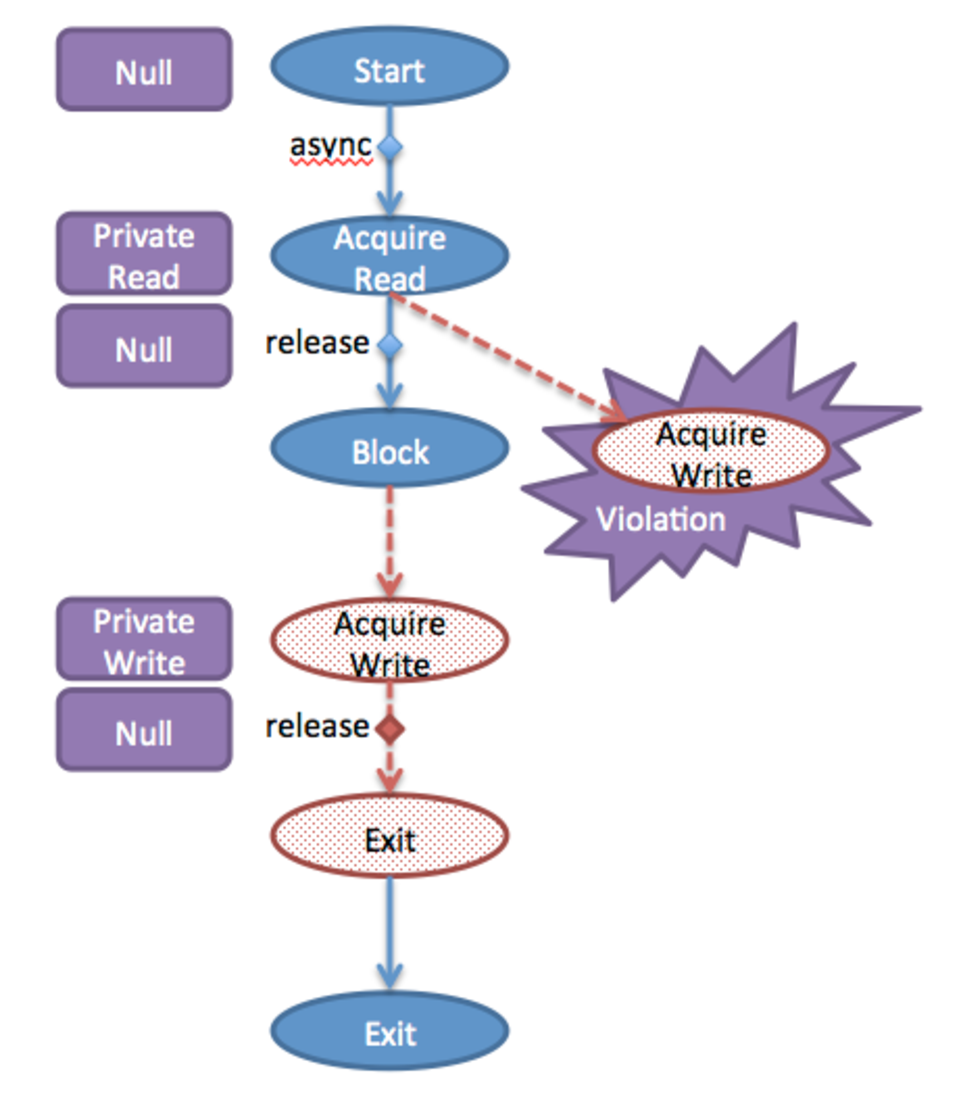
\includegraphics{../figs/stack-violation}}
  \caption{Different schedules for a permission region annotated
    version of the program in \figref{fig:hj-async-finish} with the
    schedule in the right branch reporting a permission violation.}
  \label{fig:permission-violation-state}
\end{figure}

Permission regions are programmer added annotations on shared objects
\cite{Westbrook:2011:PRR:2341616.2341627,Westbrook:2012:PPR:2367163.2367201}. The regions are indicated
as accessing shared objects in read or write mode. When the program
executes with run-time checking of permission regions enabled, a state machine is associated with each shared object to track
permissions on that object as indicated by the program annotations. If
accesses from distinct tasks on the same object conflict (i.e., a read
with a write or a write with a write), then a permission violation, indicative of a data race, is detected. An absence of violations implies an absence of any data races. 

To annotate the program in \figref{fig:hj-async-finish} with
permission regions, \lineref{line:push} and \lineref{line:peek} are
wrapped in separate regions, writing and reading, respectively, as follows:
\begin{lstlisting}
acquireW(stk);
stk.push(5);
releaseW(stk);
\end{lstlisting}
\begin{lstlisting}
acquireR(stk);
stk.peek();
releaseR(stk);
\end{lstlisting}
%Permission regions are transitive and span all the code in the
%\texttt{stk.push} and \texttt{stk.peek} methods.

The state machine associated with each region to track accesses and
detect violations is not shown due to space limitations, but it is intuitively
understood from the two possible task schedules in
\figref{fig:permission-violation-state} for an annotated version of the
program in \figref{fig:hj-async-finish}. The solid filled ovals and
solid lines represent the parent task and the dotted filled ovals and
dashed lines represent the child task created by the
\texttt{async}-statement on \lineref{line:async}. The squares indicate the current state of
the state machine that is tracking accesses to the shared object
\texttt{stk}.

The left branch of the tree is the schedule where the parent task runs
until it is blocked to wait for the child task. The parent task acquires
and releases private read privileges on the region and then the newly
created task runs, acquiring and releasing private write
privileges. If this schedule is followed in the run-time, then the
permission violation in the program is undetected. The right branch is another
possible schedule in the run-time. Here the child task runs just after
the parent task acquires private read privileges on {\tt stk}. When the
child task tries to acquire write privileges on {\tt stk}, its
state machine detects the violation.

Permission regions are distinctly different from mutual exclusion primitives such as locks and the Habanero 
\texttt{isolated}-construct. The \texttt{isolated}-construct defines
an atomic region that runs mutually exclusive to any other
\texttt{isolated}-construct and can be used to express  non-determination that is
intended by the programmer.  As such, isolated atomic regions are
serialized with respect to one another. Permission regions do not
include any serialization or synchronization semantics by themselves; rather, they check if concurrent accesses obey the permission annotations.

\begin{algorithm}
\caption{Permission Region Informed Search}\label{algo:search}
\begin{algorithmic}[1]
  \Function{search}{$t$, $h$, $T$}
  \State \textbf{loop:}\ ($h$, $T$) $:=$ \texttt{run}($t$, $h$, $T$)\label{loc:run}
  \State
  \State \textit{s} $:=$ \texttt{status}($t$, $T$)
  \State \textit{permission\_violation} = \textbf{false}
  \If{\textit{s} $=$ PR\_ENTRY} \label{loc:PR}
  \State ($h$, $T$, \textit{permission\_violation}) $:=$ \texttt{acquire}($t$, $h$, $T$)\label{loc:acquire}
  \ElsIf{\textit{s} $=$ PR\_EXIT}
  \State ($h$, $T$) $:=$ \texttt{release}($t$, $h$, $T$)\label{loc:release}
  \State \textbf{goto} loop
  \EndIf
  \State
  \If{\textit{permission\_violation}}\label{loc:datarace}
  \State report permission\_violation and exit
  \EndIf
  \State
  \State $R = $ \texttt{runnable}($T$)
  \If{$R = \emptyset$}
  \If{blocked($T$) $\neq \emptyset$}\label{loc:deadlock}
  \State report deadlock and exit
  \Else
  \State report any uncovered sharing and exit\label{loc:term}
  \EndIf
  \EndIf
  \State
  \If{$(h,T) \not\in S$}\Comment{$S$ is a global variable}\label{loc:visited}
  \State $S = S \cup \{(h, T)\}$
  \If{\textit{s} $=$ PR\_ENTRY $\vee$ \textit{s} $=$ ISOLATED}\label{loc:entry:isolated}
  \ForAll{$t_i \in R$}\label{loc:prsched}
  \State \texttt{search}($t_i$, $h$, $T$)
  \EndFor
  \Else
  \State $t_i$ := \texttt{random}($R$)\label{loc:rand}
  \State \texttt{search}($t_i$, $h$, $T$)
  \EndIf
  \EndIf
\EndFunction
\end{algorithmic}
\end{algorithm}

\section{\jpfhj\ Search Algorithm}

Permission regions create natural scheduling boundaries for model checking that can be
leveraged to mitigate state explosion while preserving the essential
behaviors of the program that lead to data races, deadlocks, assertion violations, or exceptions since they represent points of execution where sharing is expected.  The intuition is that given a fixed
program input, erroneous behavior can only arise from interactions between tasks
on shared memory. As such, it is only necessary to preempt running
tasks at the entrance to permission regions and
\texttt{isolated}-constructs. If a program has any deadlocks, data
races, assertion violations, or exceptions for a fixed program input,
then such a deadlock, data race, assertion violation, or exception exists
in one of the schedules that is explored from those preemption points.

\algoref{algo:search} is the pseudo-code for the algorithm to explore
all task schedules created at entry to permission regions and
\texttt{isolated}-constructs. The pseudo-code only covers the detection of data
races (i.e., permission region violations) or deadlocks; though, assertion violations and exceptions can be
detected similarly. The state of the program in the pseudo-code is
simplified for clarity; it is represented by a heap, $h$, and a set of
tasks, $T$. The lowercase $t$ indicates a task. \lineref{loc:run}
updates the heap and pool of tasks by running task $t$ until it
blocks, exits, reaches a permission region boundary (i.e., entry or
exit), or reaches an \texttt{isolated}-construct.

At the entry point of the permission region (PR\_ENTRY), \lineref{loc:acquire}
updates the state machine for the acquired permissions on the object in the heap and
checks to see if the acquisition signals a permission violation. At the exit
point of the permission region (PR\_EXIT), \lineref{loc:release} updates the
state machine for the released permissions on the object in the heap, and the algorithm
restarts task $t$ running anew at \lineref{loc:run}.

If there is a permission violation, then it is detected on
\lineref{loc:datarace}. Similarly, \lineref{loc:deadlock} detects a deadlock. A
deadlock state is indicated when there are no runnable tasks (i.e.,
$R = \emptyset$) and there exists tasks that are blocked. A report
for either a permission violation or a deadlock includes a witness trace for
validation and debugging. In the absence of a deadlock or a permission violation,
and when there are simply no more tasks to run, \lineref{loc:term}
terminates the search and reports any detected sharing that was not
annotated by a permission region or covered by an
\texttt{isolated}-construct. Such sharing is detected by tracking tasks on every heap access.

The set $S$ on \lineref{loc:visited} is a global set to track the
visited states. \lineref{loc:prsched} does the actual scheduling by
considering all runnable tasks, including the currently
running task $t$, as a next task to run. Note that in the current
state, if the task $t$ is preempted because it enters a permission
region, then that state reflects the acquired permissions on that
region. In the case that task $t$  blocked,
\lineref{loc:rand} chooses a random runnable task to schedule next.

\figref{fig:permission-violation-state}, shown previously, is the
state space explored by the search algorithm for the permission region
annotated version of the program in
\figref{fig:hj-async-finish}. Recall that the example has two tasks
that access the shared object {\tt stk}: one reading and the other writing. The
ovals in the diagram represent scheduling points, and as before, the
blocks on the left represent the state of the state machine tracking permissions. As
indicated by the pseudo-code, the algorithm only preempts running
tasks at the entrance to permission regions. In this example, it
schedules the child task after the main task acquires read permissions
to elicit the permission violation. By observation, if the permission regions in
the annotated program were replaced
with \texttt{isolated}-constructs, then the explored state space would
no longer include the violation, but it would include all schedules
that interleave the atomic blocks defined by the \texttt{isolated}-constructs.

\begin{algorithm}[t]
\caption{Procedure to Validate a Program}\label{algo:validate}
\begin{algorithmic}[l]
  \Procedure{validate}{$p$}
  \State ($h$, $T$) $:=$ init($p$)
  \State $R := $ runnable($T$)
  \State $t$ $:=$ random($R$)
  \State $S := \emptyset$
  \State search($t$, $h$, $T$)
  \While{uncovered sharing is reported}
  \State Add permissions or {\tt isolated} on sharing
  \State ($h$, $T$) $=$ init($p$)
  \State $S := \emptyset$
  \State search($t$, $h$, $T$)
  \EndWhile
  \EndProcedure
\end{algorithmic}
\end{algorithm}

\algoref{algo:validate} is a procedural flow describing the process of
program validation using the new search in
\algoref{algo:search}. When \algoref{algo:search}
finishes, the algorithm reports any heap locations that have been accessed by
more than one distinct task outside a permission region or an
\texttt{isolated}-construct with the input program location where that
access occurs. Using this information, a user is able to manually
annotate the program location appropriately, and then repeat the
search. The process terminates when a permission violation or a deadlock is
discovered, or no more sharing outside of permission regions or \texttt{isolated}-constructs exists.

\begin{theorem}
  \algoref{algo:search} is sound in that it only
  accepts programs that have no permission violations or deadlock on a given
  input under the restriction that the programs terminate and have all sharing correctly
  annotated with permission regions or wrapped in
  \texttt{isolated}-constructs.
\end{theorem}
\begin{proof}
The soundness proof reasons over a slightly modified version of the
algorithm that is iterative and takes as an additional input
a search tree, which is similar to \figref{fig:permission-violation-state}, that
captures all possible sequences of release and acquire statements
explored thus far. The algorithm traverses that input tree and at each
leaf node tries to extend that node by one generation if
possible. After the traversal, the algorithm returns the new tree. The
algorithm is called in an iterative manner until the tree reaches a
fix-point (which is guaranteed since the program terminates).

Let $P(n)$ be the statement that this modified search algorithm
returns all interesting sequences of acquire and release statements of
length $n$ or less for a given input program, where interesting means
containing a permission violation or deadlock.

\noindent\textbf{Basis Step:} the algorithm produces all interesting
sequences of length $n \leq 1$. This case is trivially established with
the initial state of the program that represents a sequence of length
$n \leq 1$ and cannot contain a permission violation or deadlock since the program has not yet
done anything. As such, it includes all interesting sequences.

\noindent\textbf{Inductive Step:} assume the modified algorithm has
correctly generated a tree representing all interesting sequences of $n$ or less;
it is necessary to show that from such a tree the algorithm is able to generate all
interesting sequences of length $n+1$ or less.  There are three possible outcomes at any
leaf of the input tree:
\begin{compactenum}
\item the leaf cannot be extended as it is already an interesting sequence having a permission violation or deadlock;
\item the leaf cannot be extended as there are no more tasks to run, in which case it is not interesting; or
\item the leaf is able to be extended with one or more immediate descendants.
\end{compactenum}
The first two cases are directly covered by \lineref{loc:datarace} through Line 24 of the
algorithm; there is no way to have any descendants in those
situations and the sequences are already classified as interesting or not.

For the third case, first consider \lineref{loc:entry:isolated} of the algorithm that creates
the next generation in the tree for permission regions and {\tt isolated}-constructs. Every runnable task is scheduled (\lineref{loc:prsched}) and each of those tasks
must reach an immediate successor. Such a successor may be a permission violation or a deadlock, making it an interesting sequence, a preemption, a
block condition, or exit by the constraint that the input program must
terminate. As such, any $n+1$ length sequence that exists, is
generated.

Further, any interesting $n+1$ sequence is generated. To see
this outcome, it is important to understand that the order of
acquisition relative to read or write does not matter in detecting a
violation. The state machines on the objects are not dependent on
acquisition order; they only depend on what tasks hold read or write permissions
at the time of acquisition. As the algorithm always first
acquires a permission and then schedules other tasks, it generates all
the interesting $n+1$ sequences if any exist. In this case, a sequence is interesting due to a permission violation. If a permission violation does not exist in a sequence, then a deadlock is
detected as usual.

To complete the inductive step, the code under Line 32 must be considered. That code covers
a blocked or exited task. The input program has all sharing
annotated or {\tt isolated} by the theorem statement, meaning that any non-determinism
due to scheduling is enumerated by \lineref{loc:prsched} so all reachable
program paths on the input are considered. If an interesting sequence exists
because of a deadlock, then it is either found in the $n+1$ step, by
having selected the correct task, or in a later step when the
correct task is chosen. If the deadlock depends on a particular sequence of
task executions, then those sequences are enumerated by \lineref{loc:prsched}. As
such, the deadlock is either deterministic (i.e., independent of the
schedule) or non-deterministic (i.e., a product of a data race on some
shared object). In the former, the choice of task does not matter,
and in the latter, \lineref{loc:prsched} enumerates all possible orders over permission region blocks and 
isolated blocks.
\end{proof}
As a side note, \algoref{algo:search} is complete when all regions
cover a single operation (i.e., an individual byte-code in the case of Java). Such completeness is at the cost of the number of explored schedules.

\section{Implementation and Results}
\label{sec:res}

The data race detection technique described in this paper has been implemented for Habanero Java. It uses the verification runtime specifically designed to test HJ programs \cite{anderson2014jpf}. This runtime makes use of JPF to schedule and run the programs. JPF is essentially a fully customizable Java virtual machine. JPF is modified by removing its default scheduling-factory that inserts choices on all thread actions and accesses to shared variables. Instead, a new scheduling factory based on Algorithm \ref{algo:isolated} is employed for scheduling. The computation graphs are stored in a directed acyclic graph \cite{jgrapht}. The computation graphs are exported in the dot file format for convenience and as a way to understand the structure of the program \cite{graphviz}.

The data-race detector is created by implementing the methods in the \textit{PropertyListenerAdapter} to create the computation graph. When the runtime passes an object of the type \textit{Task} to the \texttt{objectCreated} method, the \textsc{Post} rule is invoked that adds a new node to the computation graph. When the \textit{stop-finish} is executed, the \textsc{Await-next} rule is invoked that creates a node in the graph to synchronize the tasks in the finish block. The \texttt{executeInstruction} method is used to track memory locations that are accessed by various tasks by updating the node with the location accessed by the task during the execution of that instruction.

The results for this technique have been compared to two approaches implemented by JPF: \textit{Precise race detector} and \textit{Gradual permission regions} on benchmarks that cover a wide range of functionality in HJ. These two approaches are specifically chosen for comparison since the results generated by these approaches are sound for a given input just like the technique discussed in this paper. The results show a significant improvement in the time required for verification. 

The benchmarks used in this study make use of various HJ constructs for achieving task parallelism. They spawn a wide range of tasks with smaller programs having 3-15 tasks going all the way up to 525 tasks for larger programs. The experiments were run on a machine with an Intel Core i5 processor with 2.6GHz speed and 8GB of RAM.

\begin{table*}
\centering
\caption{Benchmarks of HJ programs: Computation graphs vs Permission Regions vs. PreciseRaceDetector}
\rowcolors{1}{light-gray}{white}
\label{tab:results}
\resizebox{\textwidth}{!}{
\begin{tabular}{|m{3.5cm}|c|c|c|c|c|c|c|c|c|c|c|}
\hiderowcolors
\hline
        &      &       & 
        \multicolumn{3}{c|}{\textbf{\textit{Computation graphs}}} & 
		 \multicolumn{3}{c|}{\textbf{\textit{Gradual permission regions}}} &
		\multicolumn{3}{c|}{\textbf{\textit{Precise race detector}}} \\ \hline
		
\textbf{Test ID }& \textbf{SLOC} & \textbf{Tasks} 
& \textbf{States}  & \textbf{Time}  & \textbf{Error Note }
& \textbf{States}  & \textbf{Time}  & \textbf{Error Note }
& \textbf{States}  & \textbf{Time}  & \textbf{Error Note }     \\ \hline

\showrowcolors

\textit{Primitive Array Race} & 39 & 3 
%& 5 & 00:00 & Race
& 5 & 00:00 & Race
& 5 & 00:00 & Race
& 220 & 00:00 & Race \\ \hline

\textit{Substring Search}  & 83 & 59 
%& 64 & 00:03 & Race
& 64 & 00:03 & Race
& 8 & 00:00 & Race 
& N/A & N/A & N/A \\ \hline

\textit{Reciprocal Array Sum} & 58 & 2
%& 12 & 0:00:16 & Race
& 4 & 00:08 & Race
& 32 & 00:06 & Race
& N/A & N/A & N/A \\ \hline

\textit{Primitive Array No Race} & 29 & 3 
%& 5 & 00:00 & No Race
& 5 & 00:00 & No Race
& 5 & 00:00 & No Race 
& 11,852 & 00:00 & No Race \\ \hline

\textit{Two Dim Arrays }& 30 & 11 
%& 15 & 00:01 & No Race
& 15 & 00:00 & No Race
& 15 & 00:00 & No Race 
& 597 & 00:00 & Race* \\ \hline

\textit{ForAll With Iterable} & 38 & 2
%& 9 & 00:00 & No Race
& 9 & 00:00 & No Race
& 9 & 00:00 & No Race 
& N/A & N/A & N/A \\ \hline

\textit{Integer Counter  Isolated} & 54 & 10
%& 24 & 00:01 & No Race
& 24 & 00:01 & No Race
& 1,013,102 & 05:53 & No Race 
& N/A & N/A & N/A \\ \hline

\textit{Pipeline With Futures} & 69 & 5
%& 34 & 0:00:00 & No Race
& 34 & 00:00 & No Race
& 34 & 00:00 & No Race 
& N/A & N/A & N/A \\ \hline

\textit{Binary Trees }& 80 & 525 
%& 632 & 0:00:05 & No Race
& 630 & 00:25 & No Race
& 632 & 00:03 & No Race 
& N/A & N/A & N/A \\ \hline

\textit{Prime Num Counter} & 51 & 25
%& 776 & 00:01 & No Race
& 776 & 00:01 & No Race
& 3,542,569 & 17:37 & No Race 
& N/A & N/A & N/A \\ \hline

\textit{Prime Num  Counter ForAll}  & 52 & 25
%& 30 & 0:00:02 & Race*
& 30 & 00:02 & No Race
& 18 & 00:01 & No Race
& N/A & N/A & N/A \\ \hline

\textit{Prime Num Counter ForAsync}  & 44 & 11 
%& 653 & 0:00:01 & No Race
& 653 & 00:01 & No Race
& 2,528,064 & 15:44 & No Race 
& N/A & N/A & N/A \\ \hline

\textit{Add}  & 67 & 3 
%& 11 & 0:00:01 & No Race 
& 11 & 00:01 & No Race 
& 62,374 & 00:33 & No Race
& 4930 & 00:03 & Race* \\ \hline

\textit{Scalar Multiply}  & 55 & 3 
%& 15 & 0:00:01 & No Race
& 15 & 00:01 & No Race
& 55,712 & 00:30 & No Race 
& 826 & 00:01 & Race* \\ \hline

\textit{Vector Add} & 50 & 3 
%& 5 & 0:00:01 & No Race
& 5 & 00:00 & No Race
& 17 & 00:00 & No Race 
& 46,394 & 00:19 & No Race \\ \hline

\textit{Clumped Access}  & 30 & 3 
%& 9 & 0:00:07 & No Race
& 5 & 00:03 & No Race
& 15 & 00:00 & No Race 
& N/A & N/A & N/A \\ \hline

\end{tabular}}
\vspace{-1em}
\end{table*}

\tableref{tab:results} presents the results of verification of the HJ benchmarks. The number of states explored by JPF and time required for verification by each method is compared. The tests are run for a maximum of an hour before they are terminated manually. If a test does not finish in the time bound or if it runs out of JVM memory, then it is marked as N/A in the table. The error note column shows the results of verification. The tests that produce erroneous results are marked with an asterisk ($\ast$). 

The \textit{Precise race detector} explores all potential executions of the program in a systematic way. Each execution is a sequence of transitions. Each transition takes the system from one state to another. Each transition consists of a sequence of byte-code instructions. JPF groups byte-code instructions such that an instruction that manipulates a shared variable is the first one of a transition. In every state that JPF visits, the \textit{precise race detector} checks all actions that can be performed next. If this collection of actions contains at least two conflicting accesses to a shared variable, then a data-race on the shared variable is reported. The \textit{precise race detector} inserts choices in the scheduler for all thread actions such as thread creation, synchronizations, locks etc. Therefore, it does not complete execution within the stipulated time or runs out of memory even on smaller programs because of the state space explosion. It also reports race for \textit{Two Dimensional Arrays}, \textit{Scalar multiply} and \textit{Vector Add} benchmarks where no data race actually exists in the program. This error is because in precise race detector, the access on an array object looks like a data race since it is not able to see the difference in the indexes.

\textit{Gradual permission regions} use program annotations to reduce the state space of the program \cite{mercer2015model}. Whenever a shared variable is accessed by multiple tasks in the program, the accesses have to be annotated to inform the data-race detector to create different schedules for these accesses. It is prone to human errors because of the need for manual annotation. If the program is annotated incorrectly, the results of data race detection analysis are no longer sound. \textit{gradual permission regions} works better than \textit{precise race detector}. Compared to \textit{computation graphs} in this paper though it falls behind quickly when there are several regions to annotate. A single execution is all that is needed for the \textit{computation graph analysis} while \textit{permission regions} have to enumerate an exponential number of schedules over the regions. The difference in performance is seen in the \textit{Add}, \textit{Scalar multiply} and \textit{Prime number counter} benchmarks. These benchmarks use shared variables that have to be enclosed within regions which results in a large state space for permission regions. The \textit{Prime number counter} benchmark also has isolated sections and therefore, the state space for \textit{computation graphs} is also large compared to other benchmarks.

We also evaluated our data race detector on some real world benchmarks. The \textit{Crypt-af} and \textit{Crypt-f} benchmarks are implementation of the IDEA encrytion algorithm and \textit{Series-af} and \textit{Series-f} are the Fourier coefficient analysis benchmarks adapted from the JGF suite \cite{bull2000benchmark} using \textbf{async-finish} and \textbf{future} constructs respectively. The \textit{strassen} benchmark is adapted from the  OpenMP version of the program in the Kastors suite \cite{virouleau:hal-01081974}. \tableref{tab:results1} shows the results of this evaluation.

\begin{table*}
\centering
\caption{Evaluation of Computation graphs on real world benchmarks}
\rowcolors{1}{light-gray}{white}
\label{tab:results1}
\begin{tabular}{|c|c|c|c|c|c|}
\hiderowcolors
\hline

\textbf{Test ID }& \textbf{SLOC} & \textbf{Tasks} 
& \textbf{States}  & \textbf{Time}  & \textbf{Error Note }\\ \hline

\showrowcolors

\textit{Crypt-af} & 1010 & 259
& 260 & 00:17 & No Race  \\ \hline

\textit{Crypt-f}  & 1145 & 387 
& 775 & 00:46 & No Race \\ \hline

\textit{Series-af} & 730 & 329
& 750 & 00:36 & No Race \\ \hline

\textit{Series-f} & 830 & 354 
& 630 & 00:51 & No Race\\ \hline

\textit{Strassen} & 560 & 3
& 7 & 00:57 & No Race \\ \hline

\end{tabular}
\vspace{-1em}
\end{table*}
\vspace{-2em}
\section{Related Work} \label{sec:rel-work}
Data-race detection in \emph{unstructured thread parallelism}, where there is no defined protocol for creating and joining threads, or accessing shared memory, relies on static analysis to approximate parallelism and memory accesses \cite{schonberg1989fly,choi2001static,kahlon2009static,kulikov2010detecting,vechev2011automatic} and then improves precision with dynamic analysis \cite{lamport1978time,Godefroid,flanagan2009fasttrack,EraserUpgrade,dimitrov2014commutativity}. Other approaches reason about threads individually \cite{xu1997rely,flanagan2003thread,henzinger2003thread,malkis2007precise,gotsman2007thread}, rely on  assertions \cite{burnim2009asserting, burnim2010determin, hong2012testing, yu2012maple, terragni2015recontest, yu2014simrt, leon2015unfolding, kahkonen2015unfolding}, use low-overhead instrumentation \cite{nistor2010instantcheck}, or construct type proofs \cite{abadi2006types}. These approaches  make few assumptions about the parallelism for generality and typically have higher cost for analysis. 

\emph{Structured parallelism} constrains how threads are created and joined and how shared memory is accessed through programming models. For example, a locking protocol leads to static, dynamic, or hybrid lock-set analyses for data-race detection that are typically more efficient than approaches to unstructured parallelism \cite{savage1997eraser,engler2003racerx,locksets-msr,elmas2006goldilocks,naik2006effective,elmas2007goldilocks,voung2007relay,kahlon2010universal}. Locking protocols are not directly applicable to task-parallel programming models that also constrain parallelism but often without explicit locking. 

\begin{comment}
Different types of data race detection techniques have been developed. The static race detectors analyze the source code to detect races. The dynamic ones use information from the actual program executions. Another technique for data race detection is model checking. In this method, a model of the system being analyzed is created and whether this model meets the specifications is exhaustively checked.

Static data race detectors require program instrumentation by the users. They can reason about all possible program runs. The major drawback of these systems is that they produce a large number of false-positives. \cite{engler2003racerx,ESC,abadi2006types,naik2006effective,voung2007relay,choi2001static, vechev2011automatic}. 

Dynamic race detectors use use different techniques to detect data races at runtime. The lock-set based tools track the set of locks held by each task during execution. These sets are then used to determine conflicts over shared memory references \cite{savage1997eraser, EraserUpgrade, elmas2006goldilocks, elmas2007goldilocks}. 

Dimitrov et al. developed a dynamic commutativity race detector \cite{dimitrov2014commutativity}. It uses vector clocks along with a commutativity specification to generate a structural representation of parallel programs that is used to locate races. Dynamic race detectors based on hashing asserts if different runs of a parallel program with same input produce different outputs \cite{nistor2010instantcheck}.

Lamport defined the happens-before relation in parallel programs \cite{lamport1978time}. The happens-before relation defines a partial order among all the operations in all the threads of a parallel program. The happen-before relation has been used in various data race detection techniques \cite{kahlon2009static, kahlon2010universal, flanagan2009fasttrack, mellor1991fly, schonberg1989fly, miller1988mechanism}. This approach has also been applied to task parallel languages such as Cilk and X10 \cite{Feng97efficientdetection, Async-Finish-Race}. Two approaches based on the happens-before relation, discussed in the introduction, have been developed for HJ programs \cite{raman2012scalable, drdForFutures}. 

Model checking systematically explores the entire state space of the programs to detect concurrency issues \cite{kulikov2010detecting, vakkalanka2008implementing, Godefroid}. The major drawback of model checking is the explosion in the state space as the program size increases. This technique has been extended to verify various task parallel languages such as HJ, X10 and Chapel\cite{anderson2014jpf, gligoric2012x10x, zirkel2013automated}. As opposed to model checking, predictive analysis observes only a single program execution and generalizes the verification results to all possible schedules. This approach has been applied to detecting communication deadlocks in MPI programs \cite{forejt2014precise}.

Various methods have been developed to tackle the state explosion problem of model checking. Rely-guarantee reasoning verifies threads individually using assertions about other threads \cite{xu1997rely, popeea2012compositional}. Thread modular analysis relies on a similar technique. It verifies threads individually using an abstraction of steps that may be performed by other threads \cite{flanagan2003thread, malkis2007precise, henzinger2003thread, gotsman2007thread}.

Hybrid race detection systems have been developed that combine various techniques to overcome some of the limitations of these methods. Permission regions use static program instrumentation combined with dynamic analysis to detect races \cite{westbrook2012practical, westbrook2012permission}. Gradual permission regions use a similar program instrumentation along with model checking \cite{mercer2015model}. 

This work makes use of the happens-before relation for dynamic analysis of programs and use model checking to ensure all schedules are considered in programs with mutual exclusion. A lot of different techniques create model of programs from program executions and use the models for verification. SATCheck observes the program execution to build a concrete behavior model of program execution and using a SAT solver, it tries to find other interesting behaviors \cite{demsky2015satcheck}. Coverage driven testing uses program execution to create a model of the thread interleavings and shared memory accesses to identify unexplored thread interleavings \cite{hong2012testing, yu2012maple}. Regression testing tools for concurrent programs use changes in the program model to identify shared memory accesses that might be affected by the code changes and identifying thread interleavings that must be explored to expose regression bugs \cite{terragni2015recontest, yu2014simrt}. Dynamic symbolic execution is combined with unfolding of petri-nets to create minimal test-suites for testing multi-threaded programs \cite{leon2015unfolding, kahkonen2015unfolding}.
\end{comment}

\section{Conclusion} \label{sec:conclusion}
This work presents a sound and complete technique for data race detection in task parallel programs using computation graphs.  The computation graph creation is presented with the formal semantics for task parallel languages. A scheduling algorithm to create all computation graph structures for programs containing mutual exclusion is also presented for use in model checking. The data race detection analysis is implemented for a Java implementation of the Habanero programming model using JPF and evaluated on a host of benchmarks. The results are compared to JPF's precise race detector and a gradual permission regions based extension. The results show that computation graph analysis reduces the time required for verification significantly relative to JPF's standards. 

\begin{comment}
This work can be extended in the following ways:
\begin{itemize}
\item The data race detector based on computation graphs explores just one control flow path that is taken by the program execution based on the input. The listener can be extended to explore other control flow paths by using Symbolic Execution.
\item The computation graphs can be created statically using program instrumentation and analyzed to gain performance improvements.
\end{itemize}
\end{comment}


% references section

% can use a bibliography generated by BibTeX as a .bbl file
% BibTeX documentation can be easily obtained at:
% http://www.ctan.org/tex-archive/biblio/bibtex/contrib/doc/
% The IEEEtran BibTeX style support page is at:
% http://www.michaelshell.org/tex/ieeetran/bibtex/
\bibliographystyle{IEEEtran}
% argument is your BibTeX string definitions and bibliography database(s)
\bibliography{../bib/paper-short}
%
% <OR> manually copy in the resultant .bbl file
% set second argument of \begin to the number of references
% (used to reserve space for the reference number labels box)
%\begin{thebibliography}{1}

%\bibitem{IEEEhowto:kopka}
%H.~Kopka and P.~W. Daly, \emph{A Guide to \LaTeX}, 3rd~ed.\hskip 1em plus
%  0.5em minus 0.4em\relax Harlow, England: Addison-Wesley, 1999.

%\end{thebibliography}

% that's all folks
\end{document}


